\documentclass{article}
\parskip=6pt


%\documentclass[journal=esthag,manuscript=article]{achemso}

\usepackage{authblk}
\usepackage[version=3]{mhchem}
%\usepackage{textgreek}
\usepackage{subfigure}
\usepackage[toc,page]{appendix}
                                    
\usepackage[usenames]{color}
\usepackage[colorlinks=true,
linkcolor=webgreen,
filecolor=webbrown,
citecolor=webgreen]{hyperref}
\definecolor{webgreen}{rgb}{0,.5,0}
\definecolor{webbrown}{rgb}{.6,0,0}

\usepackage{epsfig}                                                                        
\usepackage{amsmath,amssymb,amsthm,eucal}
\usepackage{amsfonts}
\usepackage{amsthm}

\newtheorem{theorem}{Theorem}
\newtheorem*{theorem*}{Theorem}
\newtheorem*{corollary}{Corollary}

\setlength{\textwidth}{6.5in}                       
\setlength{\oddsidemargin}{.1in}
\setlength{\evensidemargin}{.1in}                                              
\setlength{\topmargin}{-.5in}
\setlength{\textheight}{8.9in}
\setlength{\parindent}{0in}


\newenvironment{packed_enumerate}{
\setlength{\parsep}{0pt}
\setlength{\parskip}{0pt}
\begin{enumerate}
  \setlength{\itemsep}{0pt}
  \setlength{\parsep}{0pt}
  \setlength{\parskip}{0pt}
}{\end{enumerate}}

\newcommand\tab[1][.5cm]{\hspace*{#1}}
\usepackage[strings]{underscore}
\usepackage[margin=1cm]{caption}
\usepackage{tabularx}
\usepackage{subfigure}

% Figures- Made With Adobe Illustrator
% Figure 1: Figure1, Sample $F_7$ board and standard indexing notation
% Figure 2: Figure2..eps, Sample $E_7$ and $T_5$ boards
% Figure 3: Figure3.eps and Figure1Test3. $F_7$ board expressed in Java code
% Figure 4: Figure4.eps, Possible jumps in an $E_7$ board/display of potentialMoveSpaces
% Figure 5: Figure5.eps, Possible jumps in a $T_7% board/standard notation for $T_5$
% Figure 6: Figure6.eps, Different initial positions of $F_7$ boards
% Figure 7: Figure7.eps, Different initial positions of $E_7$ boards
% Figure 8: Figure8.eps, Different initial positions of $T_5$-$T_7$ boards
% Figure 9: Figure9.eps, SAX count in a $T_5$ board
% Figure 10: Figure10.eps, six-removal and L-removal in an $E_7$ board.
% Figure 11: Figure11.eps, "spine-count" resource count in and $E_7$ board.

\title{Peg Solitaire: A Study on Board Difficulty}

\author{Andrew D. Gramigna}

\date{June 25, 2018}

\begin{document}
\maketitle

\abstract{
Peg Solitaire is a game in which a player has a board with $M$ spaces and $M-1$ pegs and must make jumps until one peg is remaining or there are no more possible  jumps. My goal was to find a winning path for three versions of Peg Solitaire: French Solitaire, English Solitaire, and Triangular Solitaire. I did this by creating a computer program that plays until it finds a winning path, or until no more jumps are possible. I wanted to find out which version was the easiest by simulating many trials of the game where the player has no prior knowledge and is always making random jumps. I tested this on many different board types and also allowed for the \textit{initialEmptySpace} to be moved to determine if a certain space for the \textit{initialEmptySpace} provided a more favorable chance for a victory. Finally, after analyzing each case for random jumps, I incorporated a heuristic for the Triangular board $T_5$ to determine the winning percentage on this board if a player played smarter than just making random jumps.\\
\tab I found that as a whole, the French Board $F_7$ was the most difficult to solve, with in the best case a victory coming once every 7.7 million trials. Though the most difficult single board came from the English board $E_7$. With this board, the winning percentage ranged from as high as once every 17,000 games to as low as once every 100,000,000 games, depending on the location of the \textit{initialEmptySpace}. With Triangular boards, it was much easier to attain a victory, and boards with an even number of rows were easier those those with odd number of rows. On the board $T_5$, our results ranged from a victory every 146 games to one every 578 games. Incorporating a heuristic to make our program smarter when simulating a game on the Triangular board $T_5$ increased our win percentage significantly on each unique board, to as high as once every 4 games. .
}
%%%%%%%%%%%%
% Intro
%%%%%%%%%%%%
\section{Introduction}
In Peg Solitaire, we have many \textbf{spaces} that may or may not be filled by a \textbf{peg}. Spaces with a peg are considered to be \textbf{filled}, and spaces without a peg are considered to be \textbf{empty}. A \textbf{jump} is defined as a peg moving from a filed space over another filled space and into an empty space. The peg that was jumped over is then removed from the board, thus exactly one peg is removed upon the completion of each jump. French Solitaire, English Solitaire and Triangular Solitaire are different versions of Peg Solitaire, and each version is played with a different board. A \textbf{board} is a sequence of filled and empty spaces. An example of the French board is shown in Figure~\ref{fig1}, and an example of the English board and Triangular boards are shown in Figure~\ref{fig2}. The possible jumps in the French and English boards are strictly either horizontal or vertical, whereas in a Triangular board, diagonal jumps are allowed in addition to horizontal and vertical. The types of jumps in an English and French board are shown in the left section of Figure~\ref{fig4}, and the types of jumps in a Triangular board are shown in the left section of Figure~\ref{fig5}. Note that the triangular board in Figure~\ref{fig5} has more possible jumps with the only the central space as empty because of the diagonal jumps. A \textbf{victory} is attained when no more jumps can be made because there is only one peg remaining and the every other space is empty. A \textbf{loss} is attained when no more jumps can be made, but there is more than one peg remaining. A board is \textbf{solvable} if a specific sequence of jumps can result in a victory.

Throughout this paper I will be using a shorthand notation to easily specify the board by defining the type (either F, E, or T and number of rows. For example, the French board with 7 rows will be written as $F_7$. Additionally, Figure~\ref{fig1} also shows us the traditional labeling system for Peg Solitaire, which I commonly use when referring to a specific space.

\begin{figure}[htb]
\centering
%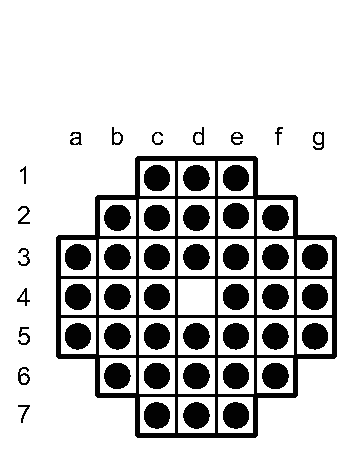
\epsfig{file=Figures/Figure1.eps}
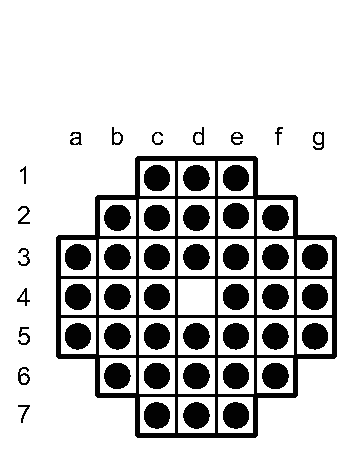
\includegraphics[width  = 5 cm]{Figures/Figure1}
\caption{Sample puzzle on the traditional 37 space French Board ($F_7$) using the traditional labeling system of the rows being numbers and the columns being letters.}
\label{fig1}
\end{figure}

\begin{figure}[htb]
\centering
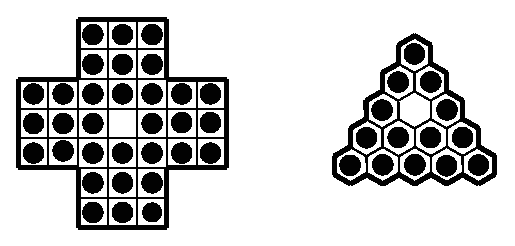
\epsfig{file=Figures/Figure2.eps}
\caption{Sample puzzles on the traditional 33 space English Board ($E_7$) and the traditional Triangular Board ($T_5$)}
\label{fig2}
\end{figure}

\section{Java Program: Random Moves Only}
Using Java I have determined winning paths for all three of these variants with variable board size which are listed in Appendix~\ref{appendix:solutions}. Traditionally, English and French Solitaire have 7 rows, whereas Triangular Solitaire has 5 (33, 37, and 21 spaces, respectively), but my program allows for the user to specify any number of rows, which I will refer to as \textbf{$N$}. It is important to note that if the user chooses a sufficiently large number for $N$, the program will not be abIe to solve the board because the generalized version of Peg Solitaire is proven to be NP-Complete~\cite{Uehara}. Of the most common boards, I found which ones are the easiest to complete and on average how many trials it will take a player making random moves achieve a victory. In my code I refer to the \textbf{\textit{initialEmptySpace}} as the space that starts out as empty when we are setting up our board in the initial state. My program allows for the \textit{initialEmptySpace} to be modified to see if a certain location makes it easier or more difficult to achieve a victory. My program consists of four classes.

\subsection{Space.java}
This class is simply defining the Space object. Each space has 3 properties, an \textit{int} for the X-value (the row), an \textit{int} for the Y-value (the column), and an \textit{int} for the status of the Space (filled, empty, or non-existent), represented by integers 1, 0, and -1 respectively. In this program I elected to use java indexing instead of the standard notation shown in  Figure~\ref{fig1} for simplicity when coding. For example, the space at ``\textit{a1}" would have the properties $x=0, y=0$ and ``\textit{e2}" would have the properties $x=1,y=4$. I have methods that allow for getting the X-value, Y-value, and status of a space, and a method for setting the status of a Space, which has the potential to alternate between filled and and empty during the course of a game.

\subsection{PSBoard.java}
\label{2.2PSBoard}
This class is a definition of the PSBoard object, which is a Peg Solitaire board viewed as a 2-D array of Spaces. To construct a board we need to define three properties, the type (Triangular, French, or English), and the number of rows/columns. This is done by adding arguments when we run the code; specifying \textit{args[0]} as ``F" and \textit{args[1]} as ``7", creates a 7x7 array of Spaces that will be initialized as a French board, meaning spaces that are not visible on the board but are present in a 7x7 square grid will have the status set to -1, so these spaces are not ever seen or used in calculations.

PSBoard.java has methods that initialize the 2-D Space array differently based on the type of the board, written as ``T", ``F", or ``E". Additionally, this class has a method that allows the users to specify the location of the \textit{initialEmptySpace}. Moving around the \textit{initialEmptySpace} allows for simulating games on different non-isomorphic boards of the same size. The row and column of the \textit{initialEmptySpace} are also specified in the command line arguments. To simulate a game of Peg Solitaire equivalent to what we have initially in Figure~\ref{fig1}, we would need to run the main class PSSim.java with the arguments \textit{F 7 3 3}, because it is a 7x7 French board with the initial empty space at $d4$. It turns out that this board is actually unsolvable~\cite{Brassine}.

\begin{figure}[htb]
\centering
\subfigure{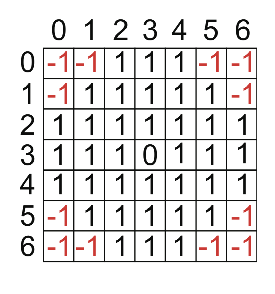
\epsfig{file=Figures/Figure3.eps}}
\hspace{.1\textwidth}
\subfigure{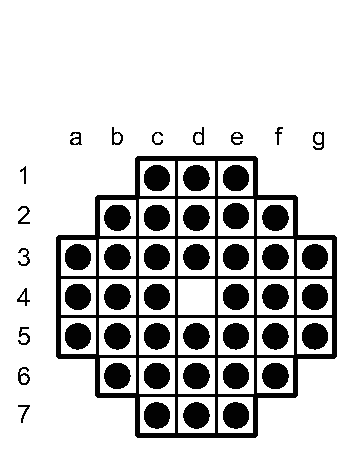
\includegraphics[width  = 4.6 cm]{Figures/Figure1}}
\caption{How the board from Figure~\ref{fig1} is represented in my Java code.}
\label{fig3}
\end{figure}

\subsection{PSGame.java}
\label{2.3PSGame}
This is the class where the actual simulation happens. We call a \textbf{trial} a series of jumps concluding with a victory or a loss. A PSGame object takes in a PSBoard object as a parameter and contains methods needed to simulate a game. We have three ArrayLists of Spaces \textit{filledSpaces}, \textit{emptySpaces}, and \textit{potentialMoveSpaces}, used to organize the status of each Space. A Space is added to \textit{potentialMoveSpaces} if and only if it is an empty Space and there a peg that can jump over another peg and into that space. Or more simply, if the requirements for a jump ending in that Space are met by at least one other peg (as shown in Figure~\ref{fig4}). The game ends when the size of \textit{potentialMoveSpaces} is zero and a victory is attained if the game ends and the size of \textit{filledSpaces} is one. These ArrayLists are updated after every move.

An important element of PSGame is the ArrayList of an array of Integers called states. Each index of states contains an Integer Array which keeps track of the status of each Space, which I call a \textbf{state}. For example, the first state of my program with arguments \textit{F 7 3 3} will be the rows Figure~\ref{fig3}, stored consecutively as a 1-Dimensional Integer Array.  After a move the new status of each peg is saved in the next state. At the end of the trial my program is able to tell each move made by noting the changes between successive states. By iterating through the states ArrayList at the end of a trial, the program able to print each unique board during our trial. Additionally, the program prints the \textbf{path} that leads us from our initial state to our final state in the traditional letter and number notation as seen in Figure~\ref{fig1}.

The most important method in this class is the move() method, which executes a jump. The move() method works through 5 simple steps:
\begin{enumerate}
\item Each space in \textit{potentialMoveSpaces} is tested determine each possible jump ending in that specific \textit{potentialMoveSpace}. Once we iterate through each space in \textit{potentialMoveSpaces}, we obtain each possible jump from the board using two ArrayLists, \textit{jumpsFrom} and \textit{jumpsTo}. Obtaining a specific index of each will match a jump. For example, if at index 3 of \textit{jumpsFrom} we have the Space representing $a3$ and at index 3 of \textit{jumpsTo} we have the Space representing $a5$, we know $a3$-$a5$ is a possible jump.
\item Out of each possible jump, we randomly select a jump to execute.
\item Once a specific jump is chosen, the jump is executed by changing the statuses of the affected spaces accordingly.
\item The ArrayLists \textit{filledSpaces}, \textit{emptySpaces}, and \textit{potentialMoveSpaces} are adjusted reflecting the changes of step 3.
\item A new jump is added to the end of our path and a new state is recorded and added to our states ArrayList.
\end{enumerate}

For an entire trial the move() method is executed continuously until we have no more moves, in which finally we test if we achieved a victory. This class has many helper methods to execute the 5 steps required for a move. 

\begin{figure}[htb]
\centering
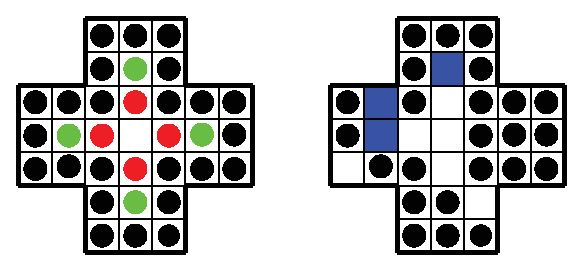
\epsfig{file=Figures/Figure4.eps}
\caption{Left: Possible jumps at the beginning of a game of an $E_7$ board. A green peg will jump over the adjacent red peg. Right: An example of a possible state later in this game. Note the blue Spaces $b3$, $b4$ and $d2$ are \textit{emptySpaces} but not \textit{potentialMoveSpaces} because there is no peg able to jump into either of these Spaces at the current state.}
\label{fig4}
\end{figure}

\begin{figure}[htb]
\centering
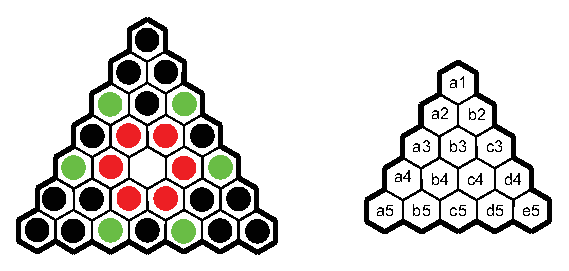
\epsfig{file=Figures/Figure5.eps}
\caption{Left: Possible jumps at the beginning of a game of an $T_7$ board. Note the two additional places to jump from in a Triangular board, $a3$ and $e7$, with \textit{potentialMoveSpace} $c5$. Right: Traditional indexing on a Triangular board ($T_5$ shown).}
\label{fig5}
\end{figure}

\subsection{PSSim.java}
This is the main method of our program. Using command line arguments, this class tells the other classes how to setup the board and initialize the spaces, states, and ArrayLists. I used this class for two separate purposes. The first was for debugging purposes, where this class would run only one trial of a Peg Solitaire game. Once everything has been initialized via the command line arguments and methods in PSBoard and PSGame, PSSim would run a single trial and print the board and path I would see if everything was working correctly and if no illegal jumps were made by testing randomly.\\
\tab The second and more important use for this class was to run many trials of the program and calculate the win percentage of a certain board. After a specified number of trials are completed, the program determines the win percentage of those trials and my results from those are shown in Section~\ref{sec3}. My program executes a Monte Carlo simulation, attempting to find the true winning percentage for various initial board states of Peg Solitaire.

%%%%%%%%%%%%
% Results
%%%%%%%%%%%%
\section{Board Difficulty: Random Moves Only}
\label{sec3}
When conducting my experiment my goals were to find a specific solution for each board, to determine the relative difficulty of each board, and to see if I can make any modifications that would improve on simply randomly guessing which jumps to execute. To find a specific solution for each board, I had the loop conducting a large number of trials terminate as soon as a winning path is found, and this path was printed to the console. Solutions to select boards can be found in Appendix~\ref{appendix:solutions}.

In order to determine which boards are easiest to solve, my program simulated play using strictly random moves. I wanted to test boards of variable type, size, and position for the \textit{initialEmptySpace}. I chose to test the most common boards $T_5$, $F_7$ and $E_7$. I also elected to test on higher $N$ triangular boards $T_6$, $T_7$, and $T_8$. I chose $T_7$ because it has the same number of rows as $F_7$ and $E_7$, and I chose $T_8$ because it has almost the same number of spaces (36) as $F_7$ (37) and $E_7$ (33). After seeing some interesting results, I also chose to test on Triangular board $T_6$. Initially, I wanted to test on higher $N$ French and English Boards, but after testing on $E_7$ and $F_7$, the win rate was so low that I did not think it would be worth diving into these higher $N$ boards, as the win rate would likely be even lower and these boards are not seen in practice anyway. Due to the incredibly low win rate for the English and French boards, I chose to simulate 100,000,000 trials for each board.

\subsection{The French Board $F_7$}
\label{3.1FrenchF7}
This was the most difficult board to simulate because of the incredibly low win rate. In the board $F_7$, there are three non-isomorphic starting positions for the empty space that allow for a solvable board ~\cite{Brassine}, shown in Figure~\ref{fig6}. All other positions are either isomorphic to these three, or represent an initial state that is already unsolvable. A non-isomorphic, solvable $F_7$ board has the \textit{initialEmptySpace} at $c1$, $d2$, or $d3$. After conducting 100,000,000 trials of strictly random jumps for each of the three unique initial positions of $F_7$, I obtained the following results:
\begin{table}[htb]
\begin{center} 
\begin{tabularx}{.88\textwidth}{ c  c  c  c  c }
\hline
\textbf{Type} & \textbf{Rows/Columns} &\textbf{Initial Empty} & \textbf{Win Rate} & \textbf{Expected Trials until Win}\\
\hline
F & 7 & c1 & $1.3*10^{-7}$ & 7,692,308\\

F & 7 & d2 & $3.0*10^{-8}$ & 33,333,333\\

F & 7 & d3 & $8.0*10^{-8}$ & 12,500,000\\

\end{tabularx}
\caption{Win rates of the three non-isomorphic $F_7$ boards. The last column is obtained by taking the floor of the number of trials divided by the number of wins.}
\label{tab1}
\end{center} 
\end{table}

\begin{figure}[htb]
\centering
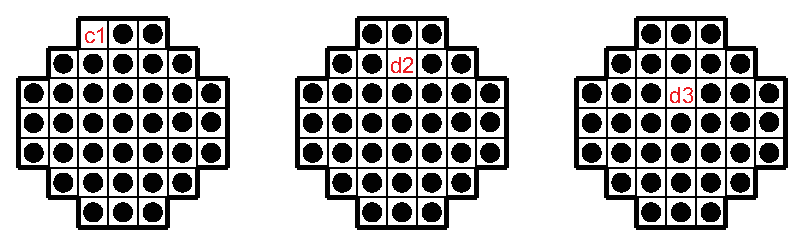
\epsfig{file=Figures/Figure6.eps}
\caption{Different initial positions of $F_7$ boards.}
\label{fig6}
\end{figure}

Immediately upon viewing Table~\ref{tab1}, we can observe that the win rate for a game of French Solitaire is incredibly low, with any of $c1$, $d2$, or $d3$ as the \textit{initialEmptySpace}. At best, with the \textit{initialEmptySpace} at $c1$, we only won 13 out of 100,000,000 games, or about 1 win every 7.7 million games. Making random moves is more or less what the average person will play, perhaps they will be more strategic towards the end if they can visualize a winning path, but prior to that they will just do random jumps much like my program. To put this into perspective, if you tried to solve the $F_7$ board with \textit{initialEmptySpace} at $c1$ 100 times a day, it would still take you over 200 years on average to solve it just once! The results show changing the \textit{initialEmptySpace} makes a victory even less likely.

It is important to note that my data for these boards is not entirely conclusive since the win rate is so low. My projected win rate could be quite different from the true win rate because each win carries such a significant weight on the end result. The goal of doing 100,000,000 trials was to try and lower the significance of each win in relation to the final winning percentage, but since the numbers are still so low, I cannot be confident that running 100,000,000 more trials would yield the same results. However, I am reasonably confident from my test an $F_7$ board with the empty space on $c1$ is slightly easier to solve than the empty space on $d3$, which is slightly easier than the empty space on $d2$. The latter of which only produced 3 wins in 100,000,000 trials. The clear takeaway, regardless of how many trials are conducted, is French Solitaire is a very difficult game to solve.


\subsection{The English Board $E_7$}
\label{3.2EnglishE7}
For the English Board , there are 7 non-isomorphic solvable starting positions, shown in Figure~\ref{fig7}. These have the location of the \textit{initialEmptySpace} at either $c1$, $c2$, $c3$, $d1$, $d2$, $d3$, or $d4$~\cite{Beasley}. After conducting 100,000,000 trials of strictly random jumps for each of the seven unique initial positions of $E_7$, I obtained the following results:



\begin{table}[htb]
\begin{center} 
\begin{tabularx}{.88\textwidth}{ c  c  c  c  c }
\hline
\textbf{Type} & \textbf{Rows/Columns} &\textbf{Initial Empty} & \textbf{Win Rate} & \textbf{Expected Trials until Win}\\
\hline
E & 7 & c1 & $6.14*10^{-6}$ & 162,866\\

E & 7 & c2 & $5.377*10^{-5}$ & 18,598\\

E & 7 & c3 & $5.875*10^{-5}$ & 17,021\\

E & 7 & d1 & $1.0*10^{-8}$ & 100,000,000\\

E & 7 & d2 & $2.06*10^{-6}$& 485,437\\

E & 7 & d3 & $3.85*10^{-6}$ & 259,740\\

E & 7 & d4 & $4.0*10^{-8}$ & 25,000,000\\
\end{tabularx}
\caption{Win rates of the unique $E_7$ boards.}
\label{tab2}
\end{center} 
\end{table}

\begin{figure}[htb]
\centering
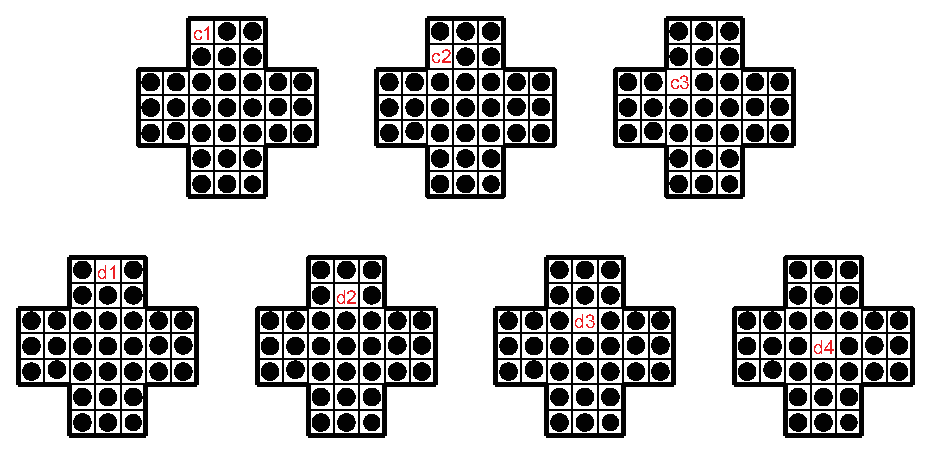
\epsfig{file=Figures/Figure7.eps, width = .88\textwidth}
\caption{Different initial positions of $E_7$ boards.}
\label{fig7}
\end{figure} 

One observation that stands out upon looking at the results on the English Board $E_7$ is the wide disparity between win rate based on the \textit{initialEmptySpace}. The low win rate is reason for caution when jumping to conclusions, but regardless of the true probabilities, it is possible to group these 7 starting positions into 5 tiers from easiest to hardest based on their win rate. The easiest tier is having the \textit{initialEmptySpace}  at $c2$ or $c3$, followed by having it at $c1$, having it at $d3$, having it at $d2$, and finally having it at $d4$ or $d1$. This is an exciting discovery because these results show there is truly a significant difference in difficulty depending on which Space is initially empty.This observation was not conclusively seen with the French Board. Simply moving the \textit{initialEmptySpace} one spot to the left, from $d1$ to $c1$, can make this puzzle 500 times easier.

The most difficult board that I tested occured when placing the \textit{initialEmptySpace} at $d1$. My program only achieved 1 win in 100,000,000 trials on this board. This is roughly the same ratio as being selected in a group of 74 people chosen from every human on Earth. English Solitaire researcher John Beasley hypothesized that this position would be the hardest to solve~\cite{Beasley}.

Overall, most positions of the English Board are significantly easier to solve than the French Board, including the three \textit{initialEmptySpaces} that were tested on both. The results show with the \textit{initialEmptySpace} in a favorable location, the 4 additional spaces in the French board $F_7$ cause such a dramatic change in win rate. This could be because the addition of these pieces in $F_7$ creates 4 new spaces that can only be reached by 2 possible jumps.

\subsection{Triangular Boards}
\label{3.3Triangular}
For the triangular boards, I tested on different values for $N$ and different positions for the \textit{initalEmptySpace}.I chose to only test on $a2$ and $a3$ for $T_7$ and $T_8$ was because $T_7$ has a very small amount of positions that are actually solvable~\cite{Bell}. Initial states with $a2$ or $a3$ are solvable on all of the four boards I tested. After conducting 100,000,000 trials of strictly random jumps for unique initial positions of various Triangular boards, I obtained the following results:

\begin{table}[htb]
\begin{center} 
\begin{tabularx}{.88\textwidth}{ c  c  c  c  c }
\hline
\textbf{Type} & \textbf{Rows/Columns} &\textbf{Initial Empty} & \textbf{Win Rate} & \textbf{Expected Trials until Win}\\
\hline
T & 5 & a1 & $0.00686670$ & 146\\

T & 5 & a2 & $0.00342621$ & 292\\

T & 5 & a3 & $0.00708800$ & 141\\

T & 5 & b3 & $0.00172991$ & 578\\

T & 6 & a1 & $0.01452690$ & 69\\

T & 6 & a2 & $0.01969780$ & 51\\

T & 6 & a3 & $0.0184591$ & 54\\

T & 6 & b3 & $0.01821328$ & 55\\

T & 7 & a2 & $8.399*10^{-5}$& 11,906\\

T & 7 & a3 & $1.2733*10^{-4}$ & 7,854\\

T & 8 & a2 & $3.3302*10^{-4}$& 3,003\\

T & 8 & a3 & $3.3189*10^{-4}$ & 3,013\\

\end{tabularx}
\caption{Win rates of the Triangular boards $T_5$-$T_8$ with various positions for the \textit{initialEmptySpace}.}
\label{tab3}
\end{center} 
\end{table}

\begin{figure}[htb]
\centering
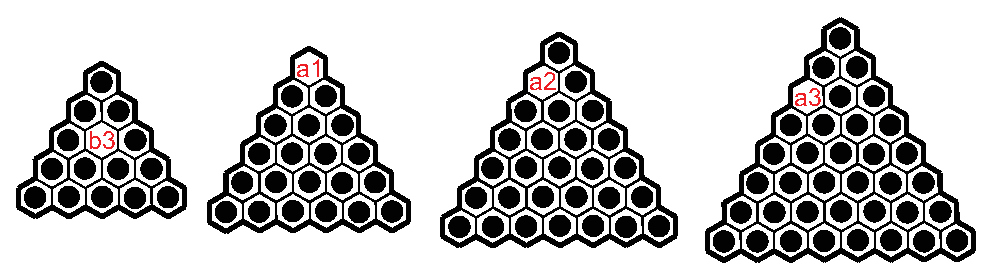
\epsfig{file=Figures/Figure8.eps, width = .88\textwidth}
\caption{$T_5$ through $T_8$ with various initial states. In all tests the \textit{initialEmptySpace} is in one of these 4 Spaces.}
\label{fig8}
\end{figure}

The most obvious observation is it much more likely to win on a triangular board than an English or French board. This is even true in the boards $T_7$ and $T_8$, which have a similar number of spaces. Perhaps this is due to the two additional jumps possible in some states of a Triangular board as shown in Figure~\ref{fig5}. Also, this could be because of the layout of the board is much more centralized, it only takes a couple jumps to go from one end of the board to the other. For the first time, with triangular boards we see that winning a game by only making random moves can be done in a reasonable amount of time, unlike the French or English boards. However once again, the location of the \textit{initialEmptySpace} makes a significant difference on how likely it is to achieve a victory, though it is not as drastic of a difference as was seen with $E_7$.\\
\tab Additionally, the results show the boards $T_6$ and $T_8$ are significantly easier to solve than their counterparts of $T_5$ and $T_7$, respectively. I expect this pattern to continue for higher values of $N$. I am confident in the validity of my program since the ``Expected Games until Victory" for the 4 unique $T_5$ boards matches with Peg Solitaire researcher George Bell's results in \textit{Solving Triangular Peg Solitaire}~\cite{Bell}.

\subsection{Analysis}
Compiling all my results when testing with random jumps, I found that Triangular boards are significantly easier to solve than the French Board $F_7$ and the English Board $E_7$. Additionally, I found that the location for the \textit{initialEmptySpace} can make a significant difference in difficultly of the board for all three types of boards. Particularly with $E_7$, the position of the \textit{initialEmptySpace} can change the difficulty of the board by a magnitude of over 5,000. For $F_7$, all three non-isomorphic boards yield an incredibly low win rate, at best we expect 1 win every 7.7 million games. For $E_7$, putting the \textit{initialEmptySpace} at $c2$ or $c3$ provide the easiest boards to solve whereas putting it at $d1$ or $d4$ provide the hardest boards to solve. For $T_5$, putting the \textit{initialEmptySpace} in the middle at $b3$ provides the most difficult board to solve, whereas putting it at $a1$ or $a3$ provides the easiest. Finally, with triangular boards, choosing an even $N$ makes the board significantly less difficult to solve than the odd row boards $N-1$ or $N+1$.
 
\section{Improving the Win Rate in the $T_5$ Board}
\label{4SAX}

Irvin and Robert Hentzel are credited with creating the \textbf{SAX Count} in the $T_5$ board. The SAX count is a useful tool in determining a solution for the $T_5$ board and it is determined as follows:\\

\begin{figure}[htb]
\centering
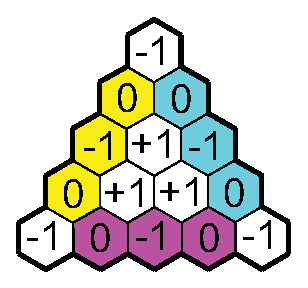
\epsfig{file=Figures/Figure9.eps}
\caption{The $T_5$ board labeled specifically to visualize the SAX count of the board.}
\label{fig9}
\end{figure}

\large S = The number of colored regions with 2 or more pegs in Figure~\ref{fig9}.\\
\tab\large A = The number pegs in spaces marked $+1$ in Figure~\ref{fig9}.\\
\tab\large X =  The number pegs in spaces marked $-1$ in Figure~\ref{fig9}.\\

\normalsize The SAX count of a board at a given state is determined by $S+A-X$~\cite{Hentzel}. It is impossible to make a jump that increases the SAX count~\cite{Bell}. Also, the lowest the SAX count can be in a solvable board is $-1$, because in order to have an SAX count less than$-1$, we must have two pegs remaining, which is not possible in a victory state. By combining these two pieces of information, we obtain:
\begin{corollary}
If the SAX count of a trial is ever below $-1$ at any state, any subsequent moves cannot result in a victory.
\end{corollary} 
Additionally, the highest possible SAX count at the initial state is 1, if we have $a1$ or $a3$ as the \textit{initialEmptySpace}. We should also note that our most difficult $T_5$ board to solve had the \textit{initialEmptySpace} at $b3$, and it is no coincidence that in this board the starting SAX count is $-1$. If we want to achieve a victory with this initial state, we cannot make a single jump that reduces the SAX count. This is very unlikely to happen when just making random jumps. The trick to improve our winning percentage, as coined by Hentzel and Hentzel, is never to make a jump that decreases the SAX count, if it can be avoided.

Obviously, this is not always possible, there are some jumps that if we make, eventually we will reach a state where we are forced make a jump which decreases the SAX count to below -1. Moreover, it is also possible to never decrease the SAX count, and still end up with 2 or more pegs remaining. However, overall, the decision to try to avoid decreasing the SAX count provides a significant increase in win percentage of the $T_5$ board, as shown in Section~\ref{4.2UpatedResults}. 
\subsection{Updates to the Program}
\label{4.1ProgramUpdates}
To incorporate the SAX count, the PSBoard and PSGame classes were updated. In PSBoard, a new method calculateSAX() was added, which calculated the SAX count at a specific state. The SAX count was only calculated if the board was a $T_5$ board. in PSGame, the move method was updated to account for the change of the SAX count. This was done by not updating the ArrayLists until we are sure of the jump we selected. We can only be sure of a jump if it does not decrease the SAX count, or it is the last possible jump we can make. The following steps were added in between steps 3 and 4 of the move() method (from Section~\ref{2.3PSGame}):
\begin{enumerate}

\item After a potential jump has been executed and the status of the Spaces has been changed, the SAX count of the state is calculated and compared with the SAX count of the previous state.
\item If the SAX count has not decreased, the ArrayLists are changed accordingly and the rest of the move() method is no different than the steps displayed in Section~\ref{2.3PSGame}.
\item If the SAX count has decreased and we are not on our last possible jump, the jump is undone, and the statuses of the spaces are changed back to the way they were before the jump was executed. The jump is removed from our two ArrayLists of possible jumps and a new jump is randomly selected from the remaining ones.
\item This process is repeated until we have found a jump that does not decrease the SAX count, or we have only one jump remaining. In the latter case, that jump is executed no matter what, because clearly none of the other jumps avoid decreasing the SAX count, leaving no option but to execute the final jump.
\end{enumerate}

With these small changes to the move() method, our program is much smarter about the jumps it makes, and this is reflected when computing the new win rate.

\subsection{Updated $T_5$ Results Adhering to the SAX Count}
\label{4.2UpatedResults}
If we repeat the experiment from Section~\ref{3.3Triangular} with the same parameters, only this time we adhere to our rule of never attempting to decrease the SAX count, our win percentage drastically improves. The results of this second version of our experiment are shown below in Table~\ref{tab4}.

\begin{table}[htb]
\begin{center} 
\begin{tabularx}{.88\textwidth}{ c  c  c  c  c }
\hline
\textbf{Type} & \textbf{Rows/Columns} &\textbf{Initial Empty} & \textbf{Win Rate} & \textbf{Expected Trials until Win}\\
\hline
T & 5 & a1 & $0.19865272$ & 5\\

T & 5 & a2 & $0.19866864$ & 5\\

T & 5 & a3 & $0.25353319$ & 4\\

T & 5 & b3 & $0.0517215$ & 19\\

\end{tabularx}
\caption{Win rates of the 4 non-isomorphic Triangular boards $T_5$ while attempting to only make jumps that don't decrease the SAX count.}
\label{tab4}
\end{center} 
\end{table}
%\newpage

\section{Future Work}
\label{5FutureWork}
\subsection{Removals}
If I were to continue looking to make improvements to my program, I would want to find a heuristic for making the French or English boards easier to solve. In his book \textit{The Ins and Outs of Peg Solitaire}, John Beasley goes over methods to make the English board ($E_7$) easier to solve. He talks about different types of \textbf{removals}, otherwise known as ways to remove a section of the board through the use of a specific sequence, without altering the rest of the board. The board must be at a certain state for these sequences to work properly~\cite{Beasley}. An example is shown in Figure~\ref{fig10}.

\begin{figure}[htb]
\centering
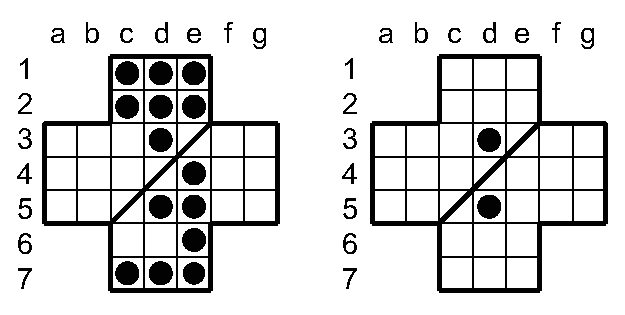
\epsfig{file=Figures/Figure10.eps}
\caption{The \textit{six-removal} and \textit{L-removal} shown.  The six-removal is shown in the top half and the L-removal in the bottom half. Left:  Our board before both removals. Right: Our board after both removals.}
\label{fig10}
\end{figure}

Note that with a specific sequence of moves we are able remove a certain section of the board without changing the status of other spaces. The sequence necessary in this example to execute a six-removal is $c1$-$c3$, $d3$-$b3$, $e1$-$c1$, $e2$-$c2$, $c1$-$c3$, $b3$-$d3$, and for the L-removal it is $d5$-$f5$, $e7$-$e5$, $e4$-$e6$, $c7$-$e7$, $e7$-$e5$, $f5$-$d5$. There are a few different states in the board where a six or L-removal is possible~\cite{Beasley}, but for simplicity I have illustrated one possible use of each in Figure~\ref{fig10}.

The six and L-removals are the most common and therefore most useful types of removals, though Beasley goes over many more that can be helpful for solving the English board. If I were to continue to make improvements to the program, I would incorporate each scenario for when one of these removals is possible into my program and have it execute the specific removal. Whether or not this would actually improve the win rate remains to be seen. Due to the complexity of this and how the addition of these removals would make the code much longer and less friendly for the average user to understand, I chose to leave it out in this version, but hope to incorporate it sometime in the future.

\subsection{Resource Counts}
A \textbf{resource count} (sometimes referred to as a pagoda function) is a function that gives a value to each space on the board and has the property that any executed jump does not increase the resource count of a state of the board. The SAX count mentioned in Section~\ref{4SAX} is a type of resource count for the $T_5$ board; this is best visualized in Figure~\ref{fig9}. There are known resource counts for the English board $E_7$~\cite{Beasley}, but their effectiveness is not as clear cut as the SAX count is for $T_5$. They are more frequently used to see if a certain jump leads to an unsolvable board later on. This phenomenon is observed if the resource count at our current state is ever less than the resource count of the intended victory state (since the resource count can never increase, we know that the victory state is not possible to reach from our current state). I chose not to incorporate a resource count for $E_7$ into my program largely because there are so many potential known resource counts to use. Incorporating the resource count would add another variable to test, being ``which resource count is the most effective at improving the win rate of an $E_7$?", and I felt that was an unnecessary distraction from my ultimate goal.

\begin{figure}[htb]
\centering
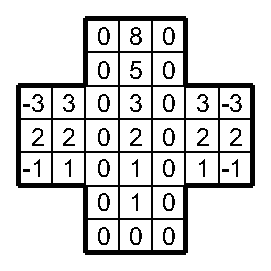
\epsfig{file=Figures/Figure11.eps}
\caption{A popular resource count for the English board $E_7$~\cite{Beasley}. The evaluation of the position of the left board in Figure~\ref{fig10} in relation to this resource count is 17, computed by adding the count of the filled spaces.}
\label{fig11}
\end{figure}

\section{Conclusion}
I created a Java program to simulate many different boards of Peg Solitaire. These boards included the French, English, and Triangular variants, with variable sizes. My program can account for any row and column size $N$, so long as they are the same and must be odd for the French version, and in this paper I did a deep dive on some of the most common sizes and variations, namely $F_7$, $E_7$, and $T_5$. Additionally, my program allows for the \textit{initialEmptySpace} to be moved around the board to test if specific locations make a difference in the difficulty to solve a board. The first version of my program determined the winning percentage of each board by only making random moves, and doing a Monte Carlo simulation with a large number of trials to get a better idea of the true winning percentage. The second version made an improvement to how my program solves the $T_5$ board making it significantly more efficient than just using random moves. The first and second version can easily be interchanged simply by commenting or uncommenting one line, as mentioned in the program.

Of the solvable boards, I found $E_7$ with the \textit{initialEmptySpace} at $d1$ the most difficult to solve, with $E_7$ with the \textit{initialEmptySpace} at $d4$ and $F_7$ with the \textit{initialEmptySpace} at $d2$ also very difficult. As a whole, of the three most common boards, $F_7$ is the most difficult to solve, followed by $E_7$, with $T_5$ being the easiest. Still, attempting to solve any $T_5$ only using random moves still yields a less than .01 success rate, while using the improvement of adhering to the SAX count, our success rate can increase to as much as .25. In the future I would like to update my program to improve the win rate of the English and French Boards as well. Specific solutions for the boards discussed in this paper can be found below in Appendix~\ref{appendix:solutions}.


\newpage
\appendix
\section{Solutions to Selected Problems} \label{appendix:solutions}
Below are some example solutions to selected boards shown in this paper. Note that these solutions are not unique, as there can be many different paths to victory from the same initial board. The format of these solutions will be the type of the board, followed by the \textit{initialEmptySpace}, followed by the path to victory. All solutions were determined by the program and double checked manually.
\subsection{$F_7$}
\subsubsection{\large $c1$}
$c3$-$c1$, $e2$-$c2$, $a3$-$c3$, $e4$-$e2$, $e6$-$e4$, $g5$-$e5$, $e4$-$e6$, $g3$-$e3$, $d3$-$f3$, $e1$-$e3$, $b2$-$d2$, $c4$-$e4$, $a4$-$c4$, $d6$-$d4$, $e4$-$e2$, $c4$-$c2$, $g4$-$e4$, $b5$-$d5$, $d1$-$d3$, $d4$-$d2$, $f2$-$f4$, $c7$-$c5$, $d5$-$b5$, $a5$-$c5$, $e7$-$e5$, $e4$-$g4$, $c1$-$c3$, $e2$-$c2$, $c2$-$c4$, $c4$-$c6$, $b6$-$d6$, $d7$-$d5$, $d5$-$f5$, $f6$-$f4$, $g4$-$e4$

\subsubsection{\large $d2$}
$f2$-$d2$, $f4$-$f2$, $e4$-$e2$, $e6$-$e4$, $f6$-$f4$, $e1$-$e3$, $c6$-$e6$, $d3$-$f3$, $g3$-$e3$, $c4$-$c6$, $e4$-$c4$, $e7$-$e5$, $d1$-$d3$, $d3$-$f3$, $c7$-$e7$, $g4$-$e4$, $e4$-$e6$, $b3$-$d3$, $a5$-$c5$, $d5$-$b5$, $b5$-$b3$, $a3$-$c3$, $c3$-$c5$, $c1$-$c3$, $d3$-$b3$, $b6$-$d6$, $e7$-$e5$, $f2$-$f4$, $b2$-$b4$, $a4$-$c4$, $c4$-$c6$, $c6$-$e6$, $e6$-$e4$, $e4$-$g4$, $g5$-$g3$

\subsubsection{\large $d3$}
$f3$-$d3$, $c3$-$e3$, $c5$-$c3$, $f5$-$f3$, $f3$-$d3$, $e4$-$c4$, $e1$-$e3$, $c7$-$c5$, $c4$-$c6$, $d5$-$f5$, $g5$-$e5$, $c2$-$c4$, $d7$-$d5$, $a3$-$c3$, $d3$-$f3$, $g3$-$e3$, $a5$-$c5$, $c4$-$c2$, $c1$-$c3$, $d5$-$f5$, $b6$-$d6$, $a4$-$c4$, $e7$-$e5$, $f6$-$f4$, $g4$-$e4$, $d1$-$d3$, $e4$-$e6$, $c4$-$c2$, $b2$-$d2$, $e3$-$c3$, $e6$-$c6$, $c6$-$c4$, $c4$-$c2$, $c2$-$e2$, $f2$-$d2$

\subsection{$E_7$}
\subsubsection{\large $c1$}
$c3$-$c1$, $e2$-$c2$, $a3$-$c3$, $b5$-$b3$, $e4$-$e2$, $e1$-$e3$, $c1$-$e1$, $c4$-$e4$, $c2$-$c4$, $e4$-$e2$, $g3$-$e3$, $e6$-$e4$, $e3$-$e5$, $g4$-$e4$, $e1$-$e3$, $d5$-$b5$, $d7$-$d5$, $e4$-$e6$, $e7$-$e5$, $a5$-$a3$, $e5$-$c5$, $g5$-$e5$, $b5$-$d5$, $c7$-$c5$, $e3$-$c3$, $c4$-$c6$, $e5$-$c5$, $c6$-$c4$, $c4$-$c2$, $a3$-$c3$, $c3$-$c1$

\subsubsection{\large $c2$}
$c4$-$c2$, $a3$-$c3$, $c6$-$c4$, $e5$-$c5$, $c4$-$c6$, $a5$-$c5$, $d3$-$d5$, $d5$-$b5$, $g5$-$e5$, $a4$-$c4$, $g3$-$g5$, $c7$-$c5$, $c4$-$c6$, $f3$-$f5$, $d1$-$d3$, $c2$-$c4$, $d7$-$d5$, $e5$-$c5$, $e3$-$c3$, $e7$-$e5$, $e4$-$e6$, $e1$-$e3$, $b5$-$d5$, $c4$-$c2$, $c1$-$c3$, $g5$-$e5$, $e6$-$e4$, $e3$-$e5$, $e5$-$c5$, $c6$-$c4$, $c4$-$c2$

\subsubsection{\large $c3$}
$a3$-$c3$, $b5$-$b3$, $d5$-$b5$, $c3$-$c5$, $b5$-$d5$, $e5$-$c5$, $d7$-$d5$, $c1$-$c3$, $e4$-$c4$, $c4$-$c2$, $g5$-$e5$, $e2$-$e4$, $d2$-$d4$, $a5$-$a3$, $d5$-$f5$, $e4$-$c4$, $e7$-$e5$, $g4$-$e4$, $g3$-$e3$, $f5$-$d5$, $e3$-$e5$, $e1$-$c1$, $c1$-$c3$, $c4$-$c2$, $c6$-$c4$, $e5$-$c5$, $a3$-$c3$, $c4$-$c6$, $c2$-$c4$, $c7$-$c5$, $c4$-$c6$

\subsubsection{\large $d1$}
$d3$-$d1$, $f3$-$d3$, $e1$-$e3$, $d3$-$f3$, $b3$-$d3$, $c1$-$e1$, $e5$-$e3$, $b5$-$b3$, $g5$-$e5$, $a3$-$c3$, $g4$-$e4$, $e4$-$e2$, $e6$-$e4$, $a5$-$a3$, $c5$-$e5$, $e1$-$e3$, $d3$-$b3$, $e4$-$e2$, $g3$-$e3$, $c7$-$c5$, $e2$-$e4$, $e4$-$e6$, $c4$-$c6$, $a3$-$c3$, $c2$-$c4$, $d4$-$b4$, $e7$-$c7$, $c7$-$c5$, $e6$-$c6$, $c6$-$c4$, $b4$-$d4$

\subsubsection{\large $d2$}
$d4$-$d2$, $f4$-$d4$, $b3$-$d3$, $c5$-$c3$, $e6$-$e4$, $c6$-$e6$, $e7$-$e5$, $a5$-$c5$, $a4$-$c4$, $d4$-$d6$, $c7$-$e7$, $c4$-$c6$, $e4$-$e6$, $d3$-$b3$, $a3$-$c3$, $d1$-$d3$, $e7$-$e5$, $d3$-$b3$, $c6$-$e6$, $e2$-$e4$, $c1$-$c3$, $g3$-$e3$, $g5$-$g3$, $b3$-$d3$, $e4$-$e2$, $e6$-$e4$, $e1$-$e3$, $d3$-$f3$, $g3$-$e3$, $e3$-$e5$, $f5$-$d5$

\subsubsection{\large $d3$}
$f3$-$d3$, $e5$-$e3$, $g5$-$e5$, $e6$-$e4$, $d3$-$f3$, $g3$-$g5$, $d1$-$d3$, $c3$-$e3$, $a3$-$c3$, $f3$-$f5$, $g5$-$e5$, $a5$-$a3$, $c6$-$e6$, $b5$-$b3$, $d4$-$b4$, $d5$-$f5$, $b3$-$d3$, $d3$-$f3$, $e1$-$e3$, $f3$-$d3$, $c1$-$c3$, $d3$-$b3$, $a3$-$c3$, $e7$-$e5$, $e4$-$e6$, $c7$-$e7$, $e7$-$e5$, $f5$-$d5$, $d5$-$b5$, $b5$-$b3$, $b3$-$d3$

\subsubsection{\large $d4$}
$f4$-$d4$, $e2$-$e4$, $c3$-$e3$, $c1$-$c3$, $e4$-$e2$, $g3$-$e3$, $d1$-$d3$, $d3$-$f3$, $g5$-$g3$, $b3$-$d3$, $d4$-$d2$, $e6$-$e4$, $c5$-$c3$, $e1$-$e3$, $e4$-$e2$, $c6$-$e6$, $a5$-$c5$, $g3$-$e3$, $d5$-$b5$, $e2$-$e4$, $a3$-$a5$, $e7$-$e5$, $e4$-$e6$, $a5$-$c5$, $c7$-$e7$, $e7$-$e5$, $f5$-$d5$, $d5$-$b5$, $b5$-$b3$, $b3$-$d3$, $d2$-$d4$

\subsection{$T_5$}
\subsubsection{\large $a1$}
$c3$-$a1$, $a3$-$c3$, $d4$-$b2$, $a1$-$a3$, $d5$-$b3$, $b5$-$d5$, $e5$-$c5$, $a4$-$a2$, $c5$-$a3$, $b2$-$b4$, $a2$-$a4$, $a5$-$a3$, $a3$-$c5$

\subsubsection{\large $a2$}
$a4$-$a2$, $c3$-$a3$, $a2$-$a4$, $c5$-$a3$, $a5$-$c5$, $a4$-$a2$, $d5$-$b5$, $a1$-$a3$, $e5$-$c3$, $b2$-$d4$, $d4$-$b4$, $b5$-$b3$, $a3$-$c3$

\subsubsection{\large $a3$}
$a5$-$a3$, $a2$-$a4$, $c3$-$a3$, $e5$-$c3$, $d5$-$b3$, $b2$-$d4$, $a4$-$a2$, $a2$-$c4$, $b5$-$d5$, $d5$-$b3$, $b4$-$b2$, $a1$-$c3$, $d4$-$b2$

\subsubsection{\large $b3$}
$d5$-$b3$, $a4$-$c4$, $b2$-$b4$, $a2$-$a4$, $b5$-$d5$, $d4$-$b2$, $a5$-$a3$, $a3$-$c5$, $d5$-$b5$, $a1$-$c3$, $c3$-$c5$, $b5$-$d5$, $e5$-$c5$

\newpage
\begin{thebibliography}{mybib} 

\bibitem{Beasley} J. Beasley, \textit{The Ins and Outs of Peg Solitaire}, Oxford University Press, 1992.

\bibitem{Brassine} M. Brassine, "D\'ecouvrez... le solitaire". \textit{Jeux et Strat\'egie}, Excelsior Publications, 1981.

\bibitem{Uehara} R. Uehara and S. Iwata, "Generalized Hi-Q is NP-complete", \textit{Trans. IEICE}, Vol. E73: 270-273, 1990.

\bibitem{Bell} G. Bell, Solving triangular peg solitaire, \textit{Journal of Integer Sequences}, Vol. 11, Article 08.4.8, 2008,\newline
\href{http://arxiv.org/abs/math/0703865}{\tt http://arxiv.org/abs/math/0703865}

\bibitem{Hentzel} I. Hentzel and R. Hentzel, Triangular puzzle peg, \textit{Journal of Recreational Mathematics}, Vol. 18, 253-256, 1986,\newline
\href{https://www.researchgate.net/publication/267664841_Triangular_puzzle_peg}
{\tt https://www.researchgate.net/publication/267664841_Triangular_puzzle_peg}

\end{thebibliography}

\end{document}